\documentclass{article}


\usepackage{siunitx} % Provides the \SI{}{} and \si{} command for typesetting SI units
\usepackage{graphicx} % Required for the inclusion of images
\usepackage{natbib} % Required to change bibliography style to APA
\usepackage{amsmath} % Required for some math elements 
\usepackage{listings}
\usepackage{placeins}
\usepackage{color}
\usepackage{caption}
\setlength\parindent{0pt} % Removes all indentation from paragraphs

\lstset{frame=tb,
  language=Matlab,
  aboveskip=3mm,
  belowskip=3mm,
  showstringspaces=false,
  columns=flexible,
  basicstyle={\small\ttfamily},
  numbers=none,
  numberstyle=\tiny\color{gray},
  keywordstyle=\color{blue},
  commentstyle=\color{green},
  stringstyle=\color{red},
  breaklines=true,
  breakatwhitespace=true,
  tabsize=3}
%\renewcommand{\labelenumi}{\alph{enumi}.} % Make numbering in the enumerate environment by letter rather than number (e.g. section 6)


\title{Lab 6 \\ Analysis of Shelf Filters }% Title

\author{Aneesh Malhotra \\ G00844135} % Author name

\date{\today} % Date for the report

\begin{document}
\maketitle % Insert the title, author and date


% If you wish to include an abstract, uncomment the lines below
% \begin{abstract}
% Abstract text
% \end{abstract}

%----------------------------------------------------------------------------------------
%	SECTION 1
%----------------------------------------------------------------------------------------

\section{Introduction}



% If you have more than one objective, uncomment the below:
\begin{description}
\item[Objective] \hfill \\
The objective of this lab was to look at shelf filters and apply them to balancing and mixing music signals.
\end{description}

\subsection{Filters}
Shelf filters alter all frequencies beyond a specific cutoff point. High shelf filters will modify all frequencies above a cutoff and low shelf filters will modify all frequencies below a specific cutoff. This can be used in balancing audio signals where a particular instrument is too loud compared to the rest. In this lab we constructed these filters, looked at their transfer functions, and applied them to various music signals.
%----------------------------------------------------------------------------------------
%	SECTION 2
%----------------------------------------------------------------------------------------

\section{Main Body}

\subsection{Low Shelf Filter}

We began by constructing a low shelf filter by constructing its transfer function. This was done by matching the coefficients using the gain and $\omega _c$ terms. We plotted the poles and zeros of this filter, as well as  response for different gain values of $g=10$ and $g= 0.1$ The plots are shown below. 


\begin{figure}[!htb]
    \centering
    \begin{minipage}{.5\textwidth}
        \centering
        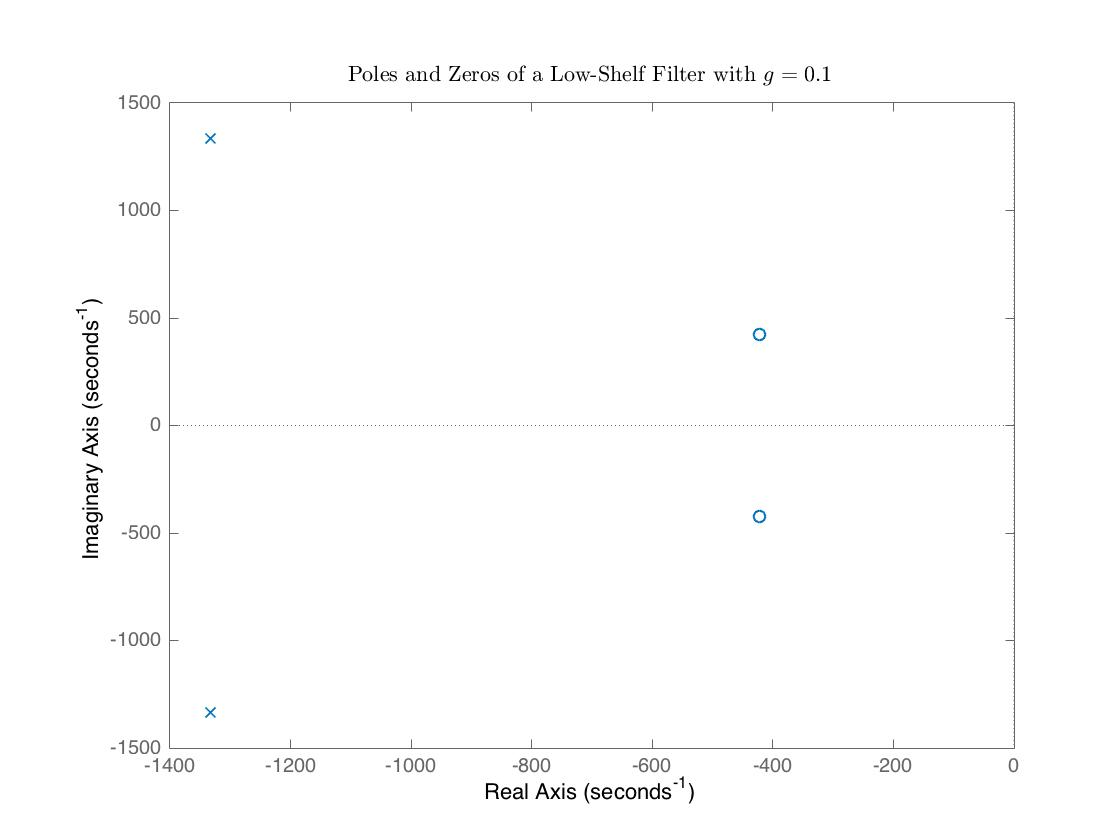
\includegraphics[width=1.0\linewidth, height=0.2\textheight]{lowshelfpoles.jpg}
        \caption{Poles and zeros of a low shelf filter with gain 0.1}
    \end{minipage}
        \begin{minipage}{.5\textwidth}
        \centering
        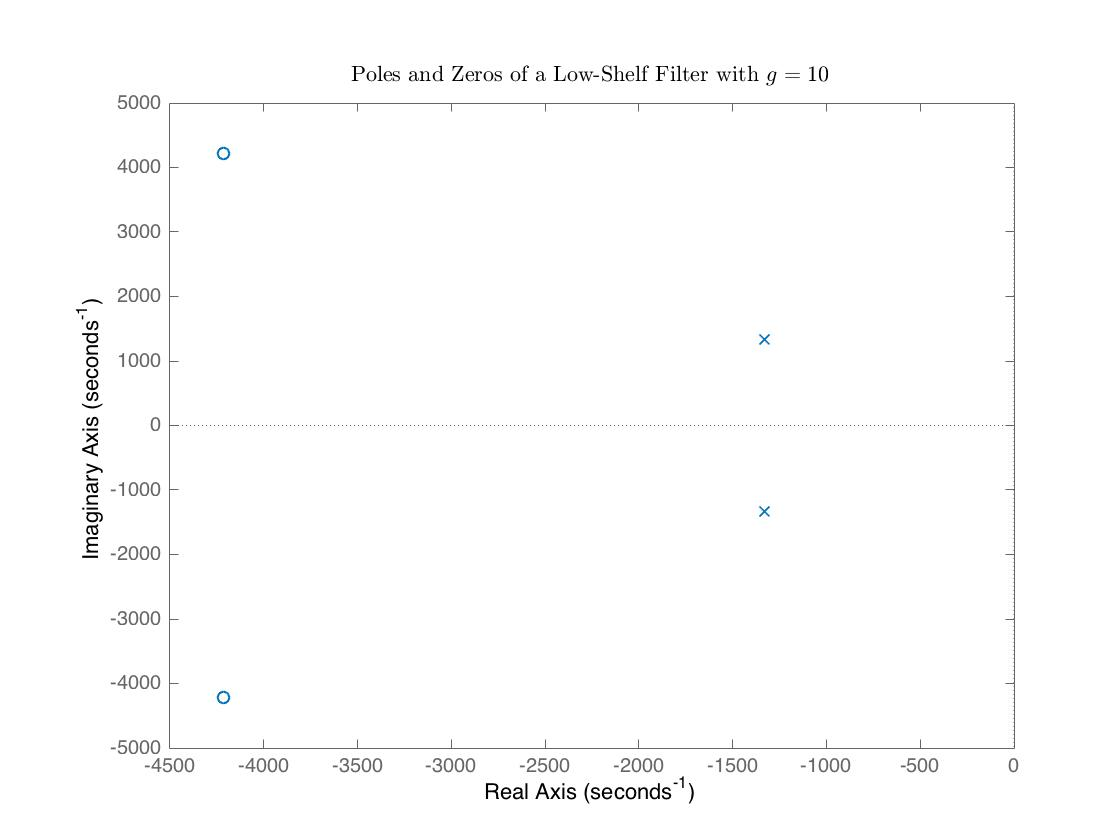
\includegraphics[width=1.0\linewidth, height=0.2\textheight]{lowshelfpoles10.jpg}
        \caption{Poles and zeros of a low shelf filter with gain 10}
    \end{minipage}
    \end{figure}
    
    
        \FloatBarrier
 We then plotted the frequency response of both of these cases:
 
 \begin{figure}[!htb]
        \centering
        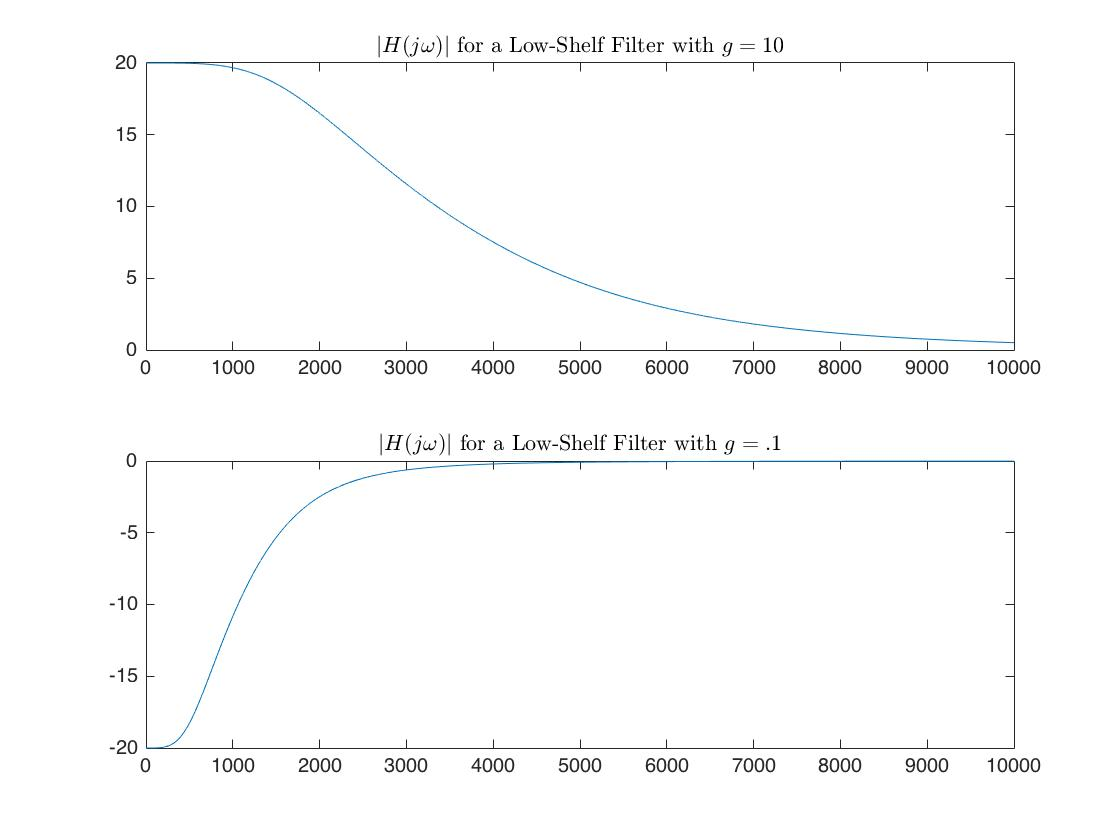
\includegraphics[width=0.6\linewidth, height=0.3\textheight]{lowshelf.jpg}
        \caption{Frequency response of a low shelf filter}
\end{figure}
\FloatBarrier
Finally, we tested this response by inputing sine waves with different inputs. The plots are given by 

 \begin{figure}[!htb]
        \centering
        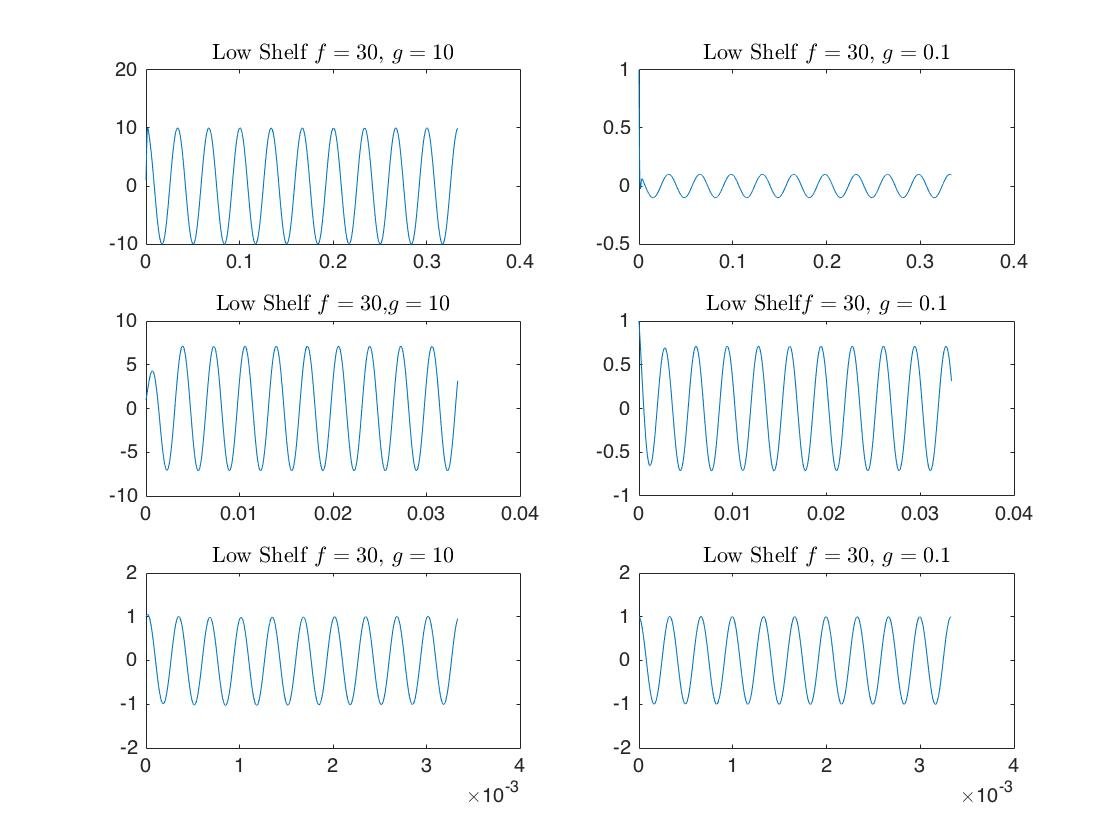
\includegraphics[width=0.8\linewidth, height=0.4\textheight]{lowsine.jpg}
        \caption{Sine inputs into a low-shelf filter}
\end{figure}
\FloatBarrier
\clearpage
\section{High Shelf Filter}
We then repeated the process above for the case of a high shelf filter using the same gain values.

\begin{figure}[!htb]
    \centering
    \begin{minipage}{.5\textwidth}
        \centering
        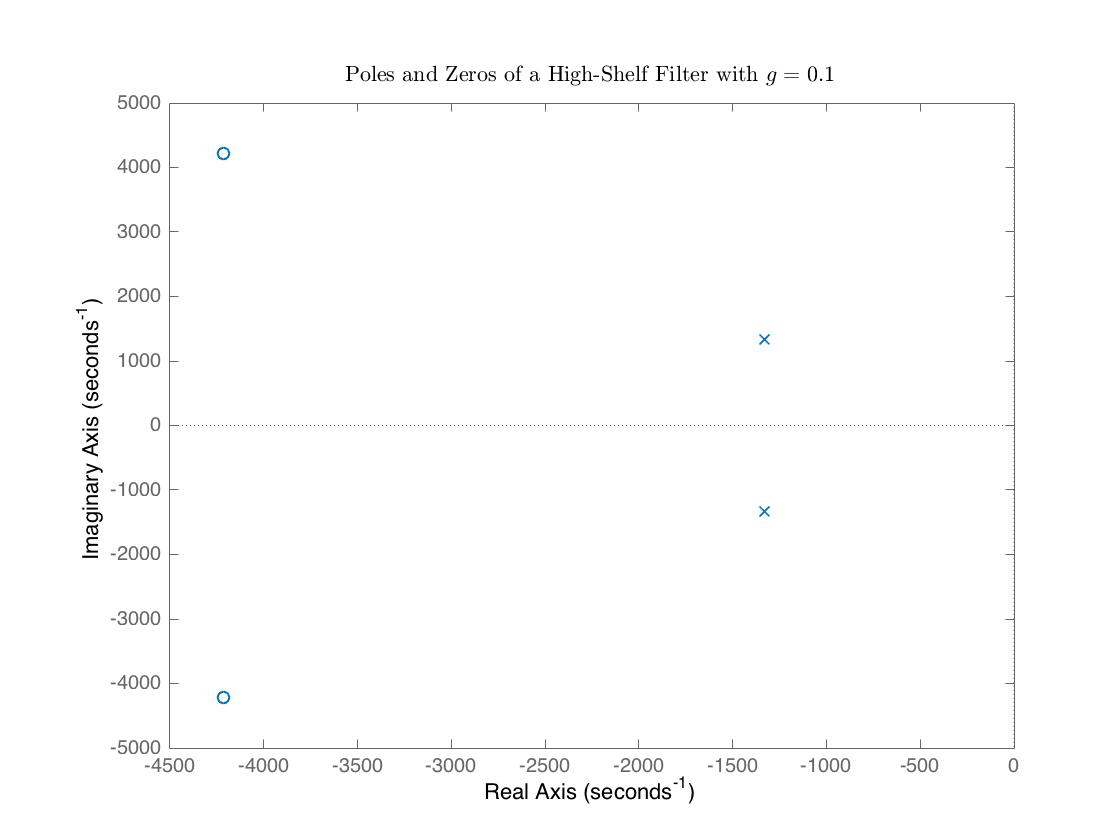
\includegraphics[width=1.0\linewidth, height=0.2\textheight]{highshelfpoles.jpg}
        \caption{Poles and zeros of a high shelf filter with gain 0.1}
    \end{minipage}
        \begin{minipage}{.5\textwidth}
        \centering
        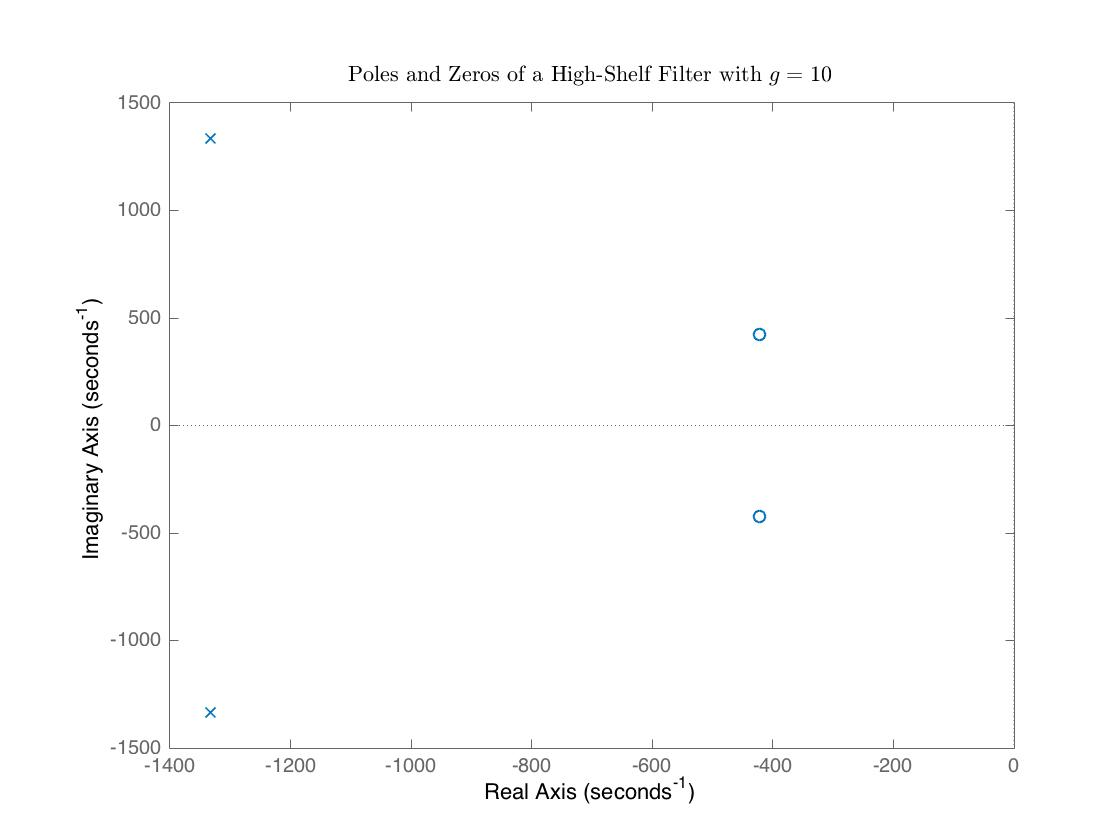
\includegraphics[width=1.0\linewidth, height=0.2\textheight]{highshelfpoles10.jpg}
        \caption{Poles and zeros of a high shelf filter with gain 10}
    \end{minipage}
    \end{figure}
    
    
        \FloatBarrier
 We then plotted the frequency response of both of these cases:
 
 \begin{figure}[!htb]
        \centering
        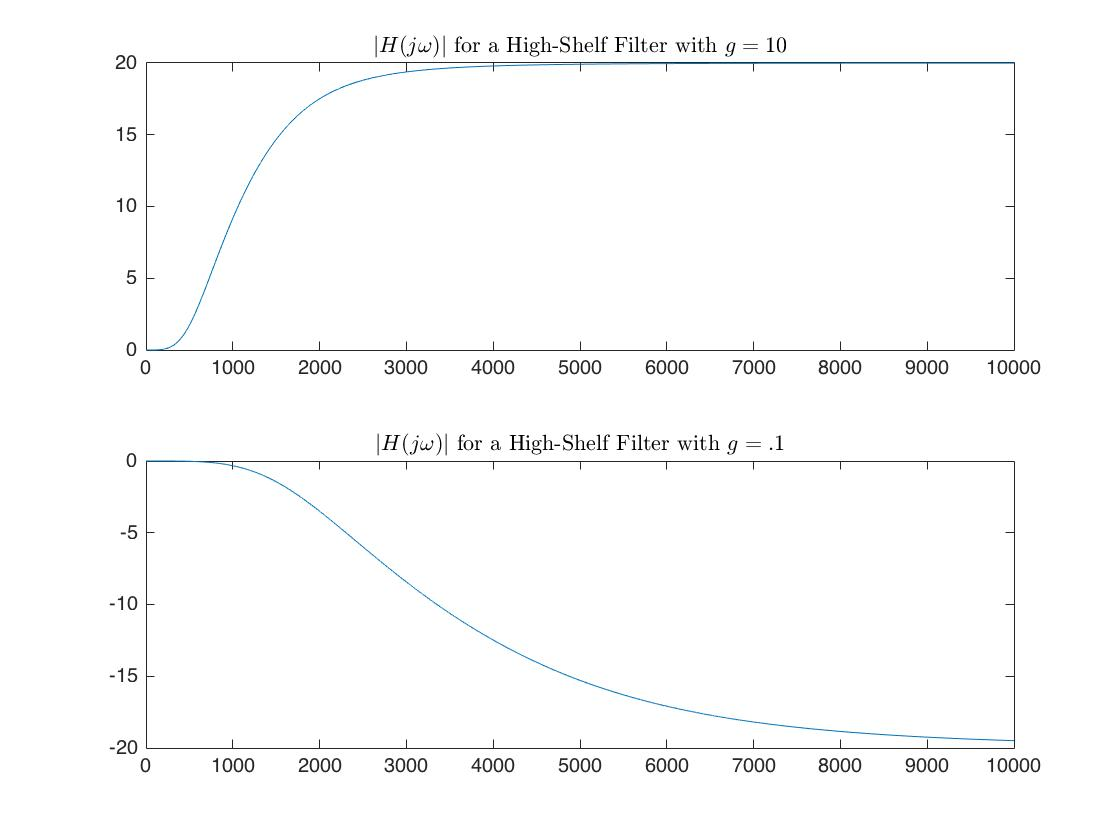
\includegraphics[width=0.6\linewidth, height=0.3\textheight]{highshelf.jpg}
        \caption{Frequency response of a low shelf filter}
\end{figure}
\FloatBarrier
Finally, we tested this response by inputing sine waves with different inputs. The plots are given by 

 \begin{figure}[!htb]
        \centering
        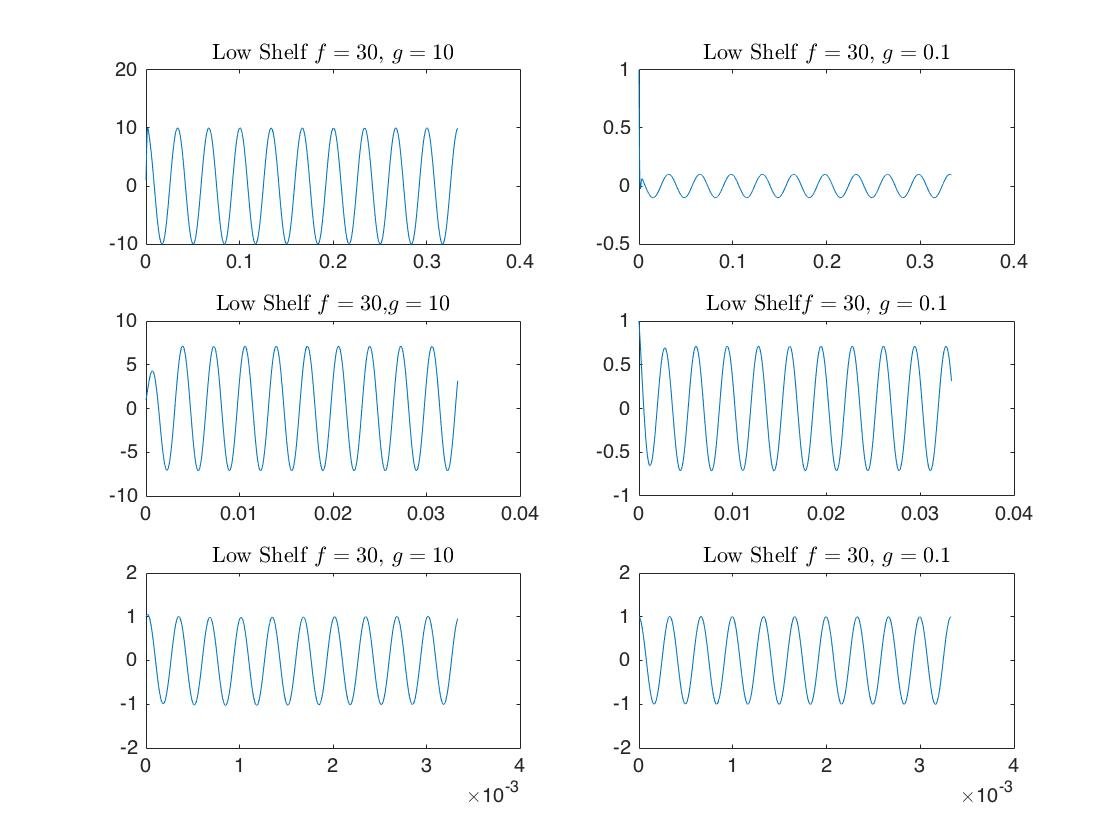
\includegraphics[width=0.8\linewidth, height=0.4\textheight]{lowsine.jpg}
        \caption{Sine inputs into a high-shelf filter}
\end{figure}
\FloatBarrier

In this case, we see we get the inverted outputs as with the low shelf case between the $g=10$ and $g=0.1$ cases. 

\section{Music Signals}
In this section we used our filter construction algorithm to design filters to alter audio signals. The first signal we looked at was the bass, piano mixture. The spectrogram of this signal is shown below:
 \begin{figure}[!htb]
        \centering
        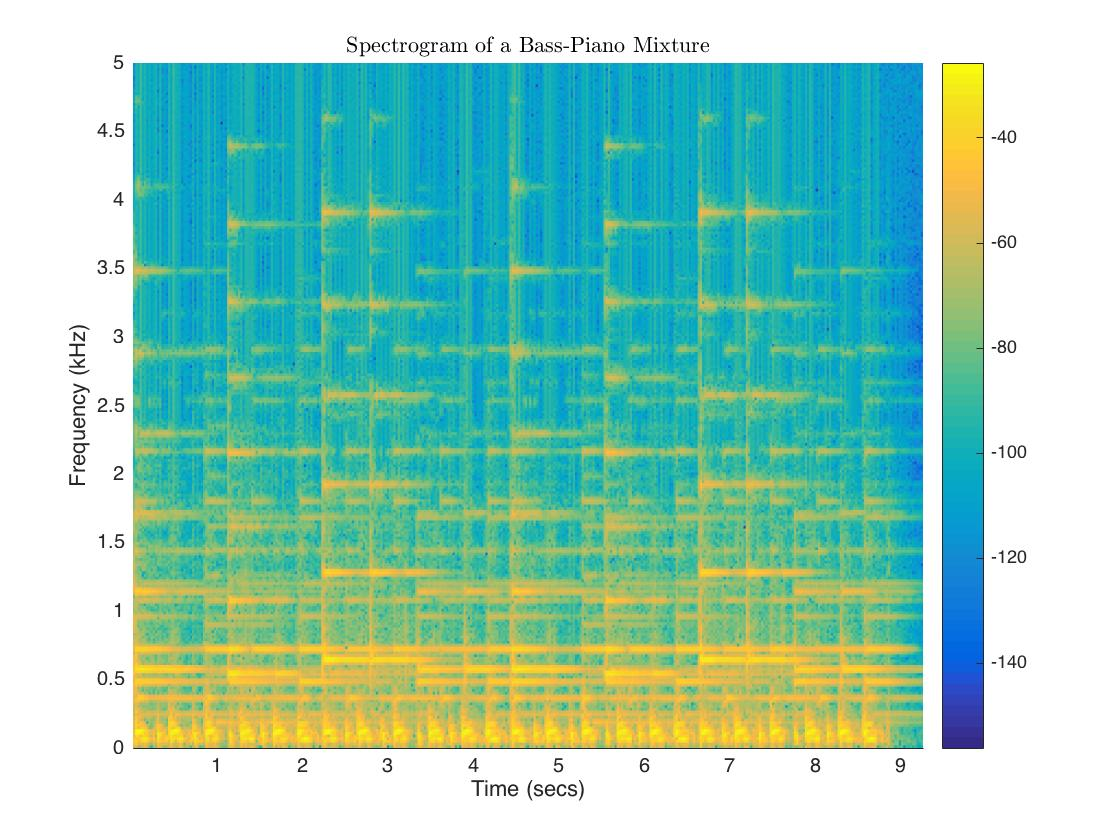
\includegraphics[width=0.6\linewidth, height=0.3\textheight]{specmixture1.jpg}
        \caption{Spectrogram of the unfiltered mixture}
\end{figure}
\FloatBarrier
We see that from this spectrogram, there is very high power in the low frequency signals. We hear this as the bass in the mixture seems to overpower the piano. In order to compensate for this, we approximated the frequency of the bass to be under 400 $\si{Hz}$. We applied a low shelf filter with a gain of 0.4 to the signal at a radian frequency of $\omega = 2\pi 400$. This reduced the bass in the mixture, as can be heard and seen in the spectrogram.

 \begin{figure}[!htb]
        \centering
        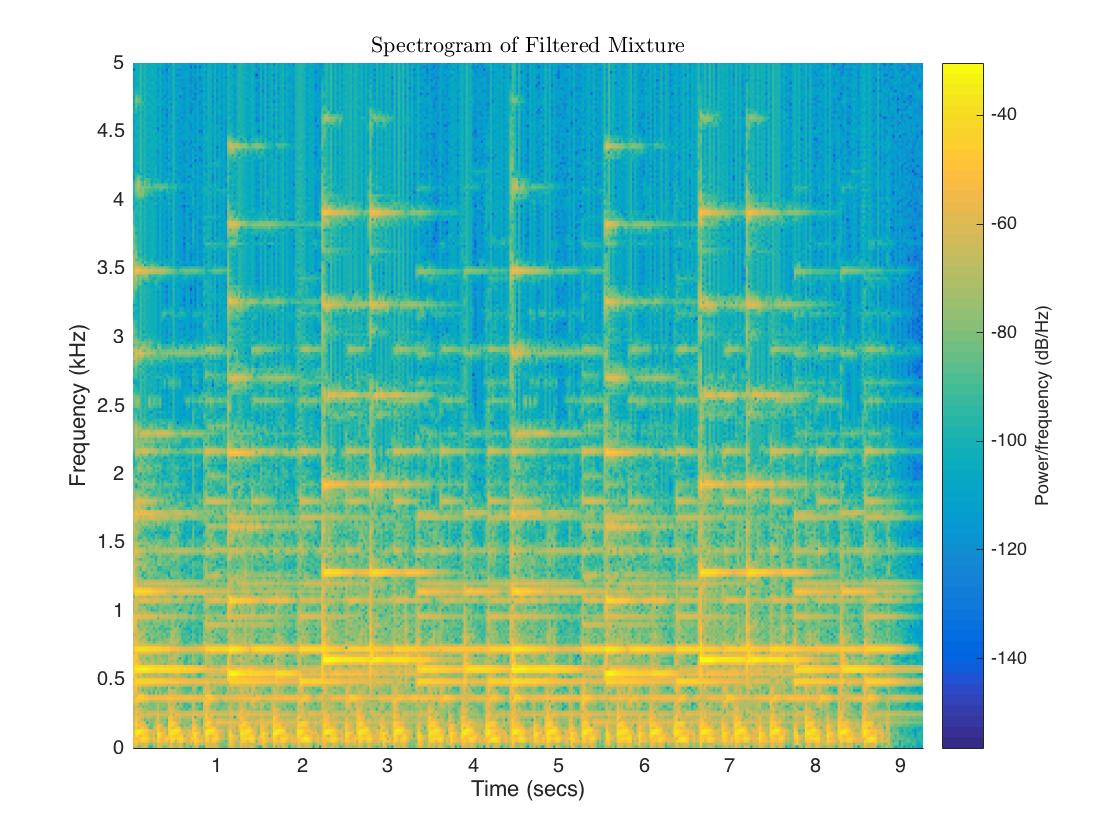
\includegraphics[width=0.6\linewidth, height=0.3\textheight]{specmixture2.jpg}
        \caption{Spectrogram of the filtered mixture}
\end{figure}

\FloatBarrier
As we can see from the filtered signal, the power of the low frequencies is much lower than initially. This can also be heard audibly using the soundsc command. Finally, we repeated this process for another music signal, which is a C-major chord played arpeggiated, and then simultaneously. Our goal was to reduce the C and E frequencies, and strengthen the G frequency. We did this by using an attenuating low shelf filter with gain 0.01 cutoff frequency at 330 $\si{Hz}$ and by passing this output signal into a high shelf filter with gain 
of 100 with cutoff frequency at 380 $\si{Hz}$. Below are the spectrograms for the original and filtered signal.

 \begin{figure}[!htb]
        \centering
        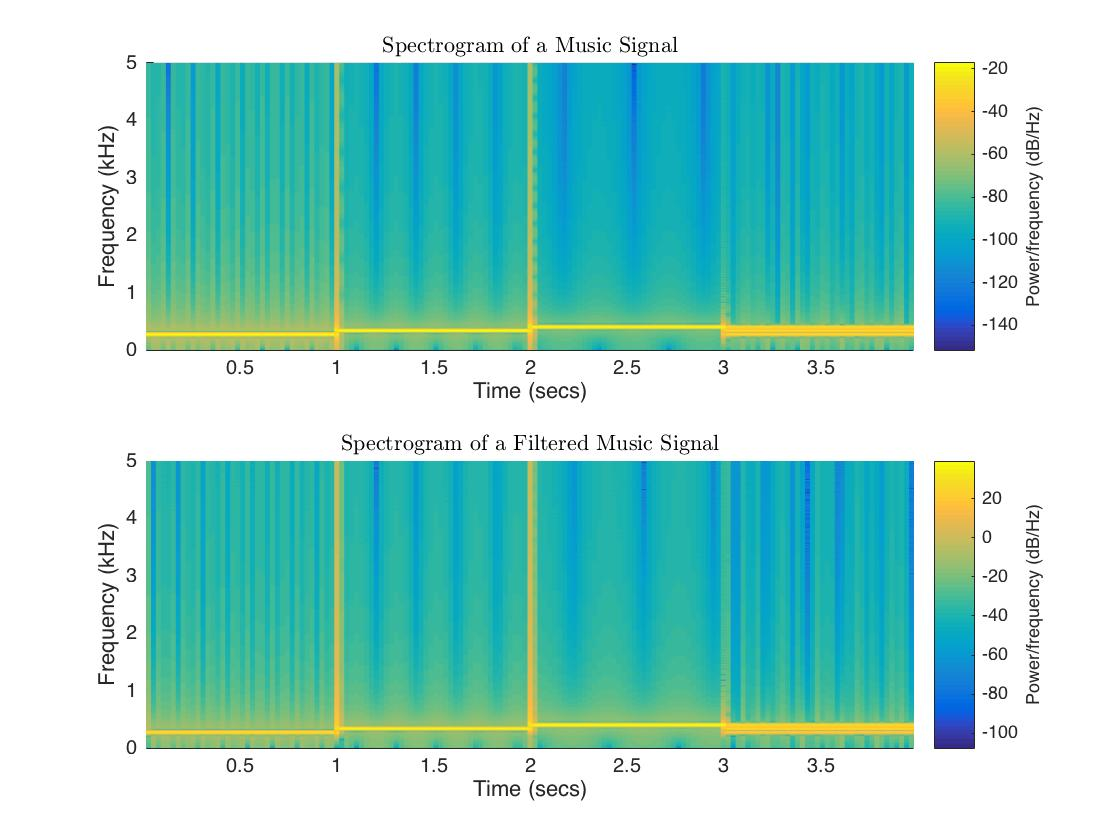
\includegraphics[width=0.6\linewidth, height=0.3\textheight]{specmusic.jpg}
        \caption{Spectrogram of a filtered and unfiltered music signal}
\end{figure}
\FloatBarrier
As we can see the spectrogram of the filtered signal has less power in the two lowest frequencies as compared to the higher frequency. This, audibly, was only slightly noticeable despite the extreme choices in gain. This is likely because we are using a non-ideal shelf filter and the choice of cutoff frequency needs to be be distant from the frequency that is actually being amplified. Additionally, the notes that were being altered were very close to each other and there may have been an overlap in the filters. 

\section{Conclusion}
In this lab we looked at shelf filters and applied them to music signals. We tend to see that low shelf filters and high shelf filters have opposing effects, and have frequency response diagrams that reflect this. When applying sinusoids of varying frequencies to these systems we saw, as expected, that in a low shelf filter, the frequencies further below the cutoff were altered, and for the high shelf the frequencies above the cutoff were altered. In the case of music, we were able to use our filter design to alter both music signals, with the case of the piano mixture to be more audibly noticeable than the chord. 
\section{Appendix}
\subsection{Lab Code}
\lstinputlisting{Lab6.m}
\subsection{Filter Function}
\lstinputlisting{design_shelf.m}
%----------------------------------------------------------------------------------------
%	BIBLIOGRAPHY
%----------------------------------------------------------------------------------------
\section{References}

Lathi, B. P. Linear Systems and Signals. New York: Oxford UP, 2005. Print.

\end{document}